\documentclass[10pt,a4paper]{article}

\usepackage{amssymb}
\usepackage[french,english]{babel}
\usepackage[utf8]{inputenc}
\usepackage{graphicx}
\usepackage{lineno}
\usepackage{cite}
\usepackage{float}
\usepackage{ccaption}
\usepackage{caption}
\usepackage{array}
\usepackage{lscape}
\usepackage[hmargin=2cm,vmargin=2cm]{geometry}
\usepackage{fancyvrb}

\title{\bf \Large A short manual for LFMM\\
\large (command-line version)
}

\author{
        Eric Frichot\\efrichot@gmail.com\\
}

\newcommand{\bp}{\mathbf{p}}
\newcommand{\LLL}{\mathcal{L}}

%% BEGIN DOC
\begin{document}

\maketitle
\begin{center}
{\it Please, print this reference manual only if it is necessary.}
\end{center}

\noindent
This short manual aims to help users to run LFMM command-line engine on Mac and Linux. 

\section{Description} 
We proposed an integrated framework based on population genetics, ecological modeling and machine 
learning techniques for screening genomes for signatures of local adaptation. We implemented fast 
algorithms using a hierarchical Bayesian mixed model based on a variant of principal component 
analysis in which residual population structure is introduced via unobserved factors. These 
algorithms can detect correlations between environmental and genetic variation at the same time 
as they infer the background levels of population structure. A description of the method is available in our paper:
\\
\\
\noindent
Eric Frichot, Sean Schoville, Guillaume Bouchard, Olivier François, 2013. {\it Landscape genomic tests for associations between loci and environmental gradients} Molecular Biology and Evolution, 30 (7), 1687-1699. 

\section{Installation} 

We provide a set of R and perl scripts and C programs to convert to LFMM format and to display manhattan plot.
By consequence, R and perl are  mandatory to display manhattan plot. 
\\
\noindent
To install LFMM CL version, you just have to execute the install script (install.sh) 
in LFMM main directory.
To execute it in a terminal shell, go to LFMM main directory and write "./install.sh".
If the script is not executable, type "chmod +x install.sh" and then "./install.sh".
A binary called \verb|LFMM| should be created in LFMM main directory.

\section{Data format}

Input files are composed of two files: a genotype file in the lfmm format and a variable file in the env format. 
\\
\\
The {\bf lfmm} format for the {\bf genotype file} has one row for each individual. Each row contains
one value per SNP (separated by spaces or tabulations): the number of alleles.
The number of alleles can be the number of reference alleles or the number
of derived alleles as long as it is the same choice for an entire SNP. The missing
genotypes are encoded with the value -9 or 9.
Here is an example with 3 individuals and 4 SNPs:
\begin{center}
\begin{Verbatim}[frame=single]
1 0 0 1
1 1 9 2
2 0 1 1
\end{Verbatim}
\end{center}

\noindent
The {\bf env} format for the {\bf variable file} has one row for each individual. 
Each row contains one value per environmental variable
(separated by spaces or tabulations).
Below, an example of variable file for $n=3$ individuals and $D=1$ covariable.
Warning: If you set several covariables, the program can be launched for each covariable sequentially
or all variables together (see command-line options).

\begin{center}
\begin{Verbatim}[frame=single]
0.252477
0.216618
-0.47509
\end{Verbatim}
\end{center}

\noindent
The {\bf zscore} format for the {\bf output file}
has one row for each SNP. Each row contains three values: The first value is the zscore, the second value is the -log10(pvalue), the third value is the p-value, the forth value is the -log10(qvalue) (based on Benjaminy-Hochberg approach) and the fifth value is the qvalue (separated by spaces or tabulations).
Below, an example of output file for $L=4$ loci.

\begin{center}
\footnotesize
\begin{Verbatim}[frame=single]
0.698819 0.314558 0.484665 0.0676981 0.855661
1.35961 0.759568 0.173953 0.224253 0.596688
0.771135 0.355929 0.440627 0.0795791 0.83257
0.879092 0.420959 0.379351 0.100315 0.793752
\end{Verbatim}
\end{center}

\section{Run the programs}
The program is executed by a command line. The format is:
\begin{Verbatim}[frame=single]
./bin/LFMM -x genotype_file -v variable_file -K latent_factors_number 
\end{Verbatim}

\noindent
All the previous options are mandatory. There is no order for the options in the command line. 
Here is a more precise description of the options:
\begin{itemize}
\item \verb|-x genotype_file| is the path for the genotype file (in {\bf lfmm} format).
\item \verb|-v variable_file| is the path for the variable file (in {\bf env} format).
\item \verb|-K latent_factor_number| is the number of latent factors. Several methods to choose $K$ are described in the tutorial. Check the references for more informations.
\end{itemize}

\noindent
Other options are not mandatory:
\begin{itemize}
\item \verb|-d nd| fit {\tt LFMM} with the nd-th variable only from the variable file. By default (if NULL and all is FALSE), fit {\tt LFMM} with each variable from the variable file sequentially and independently.
\item \verb|-a| is a boolean option. If true, fit {\tt LFMM} with all variables from the variable file at the same time. This option is not compatible with d option (by default: FALSE).
\item \verb| -o output_file| is the base of the path for the zscore output files (in {\bf zscore} format). There is one output file per environmental variable. By default, the base of the output file is the base of the name of the input file. Then it is completed with the number of the covariable (with a "a" for all and a "s" for sequentially), the number of latent factors and .zscore extension. For example, for the 3rd variable sequentially and 3 latent factors, the output file is by default input\_file\_s3.3.zscore.
\item \verb|-m| is a boolean option. If true, the input file contains missing genotypes. By default the program assumes that there is no missing data. The program is a bit slower with missing data. Please, do not use this option if it is not necessary.
\item \verb|-p p| is the number of processes (CPU) that you choose to use if you run the algorithm in 
parrallel. Be careful, the number of processes has to be lower or equal than the number of physical 
processes available on your computer. By default, the number of processes is 1.
\item \verb|-i iteration_number| is the number of iterations in the Gibbs Sampling algorithm. This number
should be large enough (by default: 1000).
\item \verb|-b burnin_number| is the number of burning iterations in the Gibbs Sampling algorithm (by default 100). 
\item \verb|-s seed| is the seed to initialize the randomization. By default, the seed is randomly chosen.
\item \verb|-C dev_file| is the path for the file containing the DIC and the deviance criterion. By default, the name of the DIC file is the name of the input file with .dic extension. 
\end{itemize}

\noindent
If you need a summary of the options, you can use the \verb|-h| option by typing the command line
\footnotesize
\begin{Verbatim}[frame=single]
./LFMM -h
\end{Verbatim}
\noindent
\normalsize

\noindent
A full example is available at the end of this note.

\section{Using {\tt LFMM} in practice}

In this section, we give practical recommendations for analyzing real data sets using the {\tt LFMM} computer program. These recommendations should help users avoiding important mistakes when using the {\tt LFMM} algorithm. Note that the following comments should not be taken too literally. Several alternative options might work equally well. 

\paragraph{Preparing the data.} Genotypic data must be prepared using the {\tt lfmm} format (any type of allelic data is allowed). The {\tt LFMM} program can handle missing data, but the algorithm used for genotype imputation is basic. We encourage users having more than $10\%$ missing genotypes in their data to fix the missing data issue by using {\it matrix completion} or {\it genotype imputation} programs such as {\tt IMPUTE2} or {\tt MENDEL-IMPUTE} before starting their analyses with {\tt LFMM}. 
Ecological data must be prepared using the {\tt env} format. To decide which variables should be used among a large number of ecological indicators (eg, climatic variables), we suggest that users summarize their data using linear combinations of those indicators.  Considering principal component analysis (or similar approaches) and using the first components as new ecological variables is one of these approaches.

\paragraph{Setting run parameters.}  The {\tt LFMM} program is based on a stochastic algorithm (MCMC) which cannot provide exact results. We recommend using large number of cycles (e.g., {\tt -i 10000}) and the burn-in period should set at least to one-half of the total number of cycles ({\tt -b 5000}). We have noticed that the program results are sensitive to the run-length parameter when data sets have relatively small sizes (eg, a few hundreds of individuals, a few thousands of loci). We recommend increasing  the burn-in period and the total number of cycles in this situation.        

\paragraph{Deciding the number of latent factors.} Deciding an appropriate value for the number of latent factors in {\tt LFMM} can be based on the analysis of histograms of test $p$-values. Here, the objective is to control the false discovery rate while keeping reasonable power to reject the null hypothesis.  To choose the number of factors, we suggest using the genomic inflation factor. According to Devlin and Roeder (1999), this quantity is defined  as 
$$
\lambda = {\rm median}( z^2 ) /0.456 \, . 
$$
The inflation factor usually decreases with increasing values of $K$. To compute the genomic inflation facto, we recommend using several runs for each value of $K$ and taking the median or the mean of the  $\lambda$ values obtained from the above formula (use 5 to 10 runs, see our script below).  Choosing values of $K$ for which the estimate of $\lambda$ is close to (or slightly below) 1.0 warrants that the FDR can be controlled efficiently. 

Testing all $K$ values in a large range, from 1 to 20 for example,  is generally useless. A careful analysis of population structure and estimates of the number of ancestral populations contributing to the genetic data indicates the range of values to be explored. If for example the {\tt sNMF} or {\tt ADMIXTURE} programs estimate 5 ancestral populations, then running {\tt LFMM} $K = 4-7$ often provides inflation factors close to 1.0.  

\paragraph{Combining $z$-scores obtained from multiple runs.}  We suggest using the Fisher-Stouffer or a similar method to combine $z$-scores from multiple runs. In practice, we found that using the median $z$-scores of 5-10 runs and re-adjusting the $p$-values afterwards increase the power of {\tt LFMM} tests. This can be done by using the following sequence of {\tt R} commands. Assuming that results from 5 runs with a particular value of $K$ are recorded in external files named {\tt zscore.res1}, {\tt zscore.res2}, etc, we can compute $p$-values using the the following commands   
{\tt 

z.table = NULL

for (i in 1:5)\{ 
 
file.name = paste("zscore.res",i, sep="")

z.table = cbind(z.table, read.table(file.name)[,1])

\}
    
z.score = apply(z.table, MARGIN = 1, median)
      
lambda = median(z.score\^~2) /0.456

p.values = pchisq(z.score\^~2 / lambda, df = 1, lower = F))

}        
                        
                        
                        
\noindent For an expected value of the FDR equal to $q$  (set $q= 10 \%$ or $q = 15 \%$), a list of candidate loci stored in the object {\tt candidate} can be obtained by using the Benjamini-Hochberg procedure as follows
 {\tt

  L = length(p.values) 
  
  n = sum( sort(p.values) < q*(1:L)/L )
  
  candidates = which( p.values < q*n/L )

}

%\section{How to choose $K$, the number of latent factors}
%The number of latent factors is the number of principal components (or latent factors) that is
%required to describe the neutral structure of the data. Several values should be tested.
%A too small value of $K$ leads to liberal tests and may generate False Positive results.
%A too large value of $K$ leads to conservative tests and may generate False Negative results.           
%We advise you to be really careful in the choice of $K$ and to test several values of $K$.
%
%\subsection{based on a population structure analysis}
%\paragraph{with a Principal Component Analysis approach}
%In our paper, we used the number of significative principal components in the
%Tracy-Widom test of {\tt SmartPCA} (http://helix.nih.gov/Applications/eigensoft.html)
%\cite{Patterson_2006}. This heuristic may be a bit too conservative.
%
%\paragraph{with on a clustering approach}
%We also used the Bayesian clustering programs {\tt STRUCTURE}\\
%(http://pritch.bsd.uchicago.edu/software/structure2\_1.html) \cite{Pritchard_2000}, {\tt TESS}\\
%(http://membres-timc.imag.fr/Olivier.Francois/tess.html) \cite{Chen_2007, Durand_2009} and
%{\tt sNMF} (a fast program to estimate ancestry coefficients) \\
%(http://membres-timc.imag.fr/Olivier.Francoissnmff.html)
%to find K the number of components which could better describe our simulated data.
%
%\subsection{based on p-values distribution}
%coming soon...
%
%\section{variance}
%coming soon an explanation of the percentage of variance explained by each variable.

\section{Annex programs}

We provide a set of R and perl scripts and C programs convert to LFMM format and to plot manhattan plot.

\subsection{Data Format}
Input files are composed of two mandatory files (a genotype file and an environmental variable file)
and one optional file (the snp information file). The snp file is interesting to analyze zscore
results and display results with manhattan plots.
It is not necessary to provide information about individuals.
All data formats are described with the same
example. These files are available in \verb|examples/format_example/|.

\subsubsection{Genotype Data}
\begin{itemize}
\item lfmm (example.lfmm)\\
The {\bf lfmm} format has one row for each individual. Each row contains
one value per SNP (separated by spaces or tabulations): the number of alleles.
The number of alleles can be the number of reference alleles or the number
of derived alleles as long as it is the same choice for an entire SNP. The missing
genotypes are encoded with the value -9 or 9.

\begin{center}
\footnotesize
\begin{Verbatim}[frame=single]
1 0 0 1
1 1 9 2
2 0 1 1
\end{Verbatim}
\end{center}

\item ped (example.ped) \\
The {\bf ped} format has one row for each individual. Each row contains 6 columns of information for each individual, plus two genotype columns for each SNP. Each column must be separated by spaces or tabulations. The genotype format must be either 0ACGT or 01234, where 0 means missing genotype. The first 6 columns of the genotype file are: the 1st column is the family ID, the 2nd column is the sample ID, the 3rd and 4th columns are the sample IDs of parents, the 5th column is the gender (male is 1, female is 2), the 6th column is the case/control status (1 is control, 2 is case), the quantitative trait value or the population group label.

The ped format is described here: http://pngu.mgh.harvard.edu/~purcell/plink/data.shtml.

\begin{center}
\footnotesize
\begin{Verbatim}[frame=single]
1       SAMPLE0 0 0 2 2 1 2 3 3 1 1 2 1
2       SAMPLE1 0 0 1 2 2 1 1 3 0 4 1 1
3       SAMPLE2 0 0 2 1 2 2 3 3 1 4 1 2
\end{Verbatim}
\end{center}

\item ancestrymap (example.ancestrymap)\\
The {\bf ancestrymap} format has one row for each genotype. Each row has 3 columns: the 1st column is the SNP name, the 2nd column is the sample ID, the 3rd column is th number of alleles. It is assumed that the genotypes for a given SNP name are written in consecutive lines. It is also assumed that the genotypes for a set of individuals are given in the same order as lines. The number of alleles can be the number of reference alleles or the number of derived alleles as long as it is the same choice for an entire SNP. It is assumed that the missing genotypes are encoded with the value 9.
\begin{center}
\footnotesize
\begin{Verbatim}[frame=single]
              rs0000              SAMPLE0   1
              rs0000              SAMPLE1   1
              rs0000              SAMPLE2   2
              rs1111              SAMPLE0   0
              rs1111              SAMPLE1   1
              rs1111              SAMPLE2   0
              rs2222              SAMPLE0   0
              rs2222              SAMPLE1   9
              rs2222              SAMPLE2   1
              rs3333              SAMPLE0   1
              rs3333              SAMPLE1   2
              rs3333              SAMPLE2   1
\end{Verbatim}
\end{center}

\item geno (example.geno)\\
The {\bf geno} format has one row for each SNP.
Each row contains 1 character per individual:
        0 means zero copy of the reference allele.
        1 means one copy of the reference allele.
        2 means two copies of the reference allele.
        9 means missing data.

\begin{center}
\footnotesize
\begin{Verbatim}[frame=single]
112
010
091
121
\end{Verbatim}
\end{center}

\item vcf (example.vcf)\\
The {\bf vcf} The vcf format is described here\\
http://www.1000genomes.org/wiki/Analysis/Variant\%20Call\%20Format/vcf-variant-call-format-version-41

\begin{center}
\footnotesize
\begin{Verbatim}[frame=single]
##fileformat=VCFv4.1
##FORMAT=<ID=GM,Number=1,Type=Integer,Description="Genotype meta">
##INFO=<ID=VM,Number=1,Type=Integer,Description="Variant meta">
##INFO=<ID=SM,Number=1,Type=Integer,Description="SampleVariant meta">
#CHROM POS ID REF ALT QUAL FILTER INFO FORMAT SAMPLE0 SAMPLE1 SAMPLE2
1 1001 rs0000 T C 999 . VM=1;SM=100 GT:GM 1/0:1 0/1:2 1/1:3
1 1002 rs1111 G A 999 . VM=2;SM=101 GT:GM 0/0:6 0/1:7 0/0:8
1 1003 notres G AA 999 . VM=3;SM=102 GT:GM 0/0:11 ./.:12 0/1:13
1 1004 rs2222 G A 999 . VM=3;SM=102 GT:GM 0/0:11 . 1/0:13
1 1003 notres GA A 999 . VM=3;SM=102 GT:GM 0/0:11 ./.:12 0/1:13
1 1005 rs3333 G A 999 . VM=3;SM=102 GT:GM 1/0:11 1/1:12 0/1:13
\end{Verbatim}
\end{center}


\end{itemize}
{\it Tips:} As LFMM does not model allele frequencies, genotype file can be
the number of copy of either the reference allele or the derived allele.

\subsubsection{Snp Data}
Warning: SNP data information has to be in the same order as in genotypic data file.

\begin{itemize}
\item pedsnp (example.pedsnp or example.map) \\
The snp file contains 1 line per SNP.  There are 6 columns (last 2 optional):
  1st column is chromosome.  Use X for X chromosome,
  2nd column is SNP name,
  3rd column is genetic position (in Morgans),
  4th column is physical position (in bases),
  Optional 5th and 6th columns are reference and variant alleles.

\begin{center}
\footnotesize
\begin{Verbatim}[frame=single]
11       rs0000     0.000000            0 A C
11       rs1111     0.001000       100000 A G
11       rs2222     0.002000       200000 A T
11       rs3333     0.003000       300000 C A
\end{Verbatim}
\end{center}

\item snp (example.snp) \\
The snp file contains 1 line per SNP.  There are 6 columns (last 2 optional):
  1st column is SNP name,
  2nd column is chromosome.  Use X for X chromosome,
  2nd column is SNP name,
  3rd column is genetic position (in Morgans)  (If unknown, ok to set to 0.0),
  4th column is physical position (in bases),
  Optional 5th and 6th columns are reference and variant alleles.
\begin{center}
\footnotesize
\begin{Verbatim}[frame=single]
              rs0000  11        0.000000               0 A C
              rs1111  11        0.001000          100000 A G
              rs2222  11        0.002000          200000 A T
              rs3333  11        0.003000          300000 C A
\end{Verbatim}
\end{center}

\item lfmmsnp (example.lfmmsnp) \\
The snp file contains 1 line per SNP.  There are 3 columns:
  1st column is SNP name,
  2nd column is chromosome,
  3th column is physical position (in bases).
\begin{center}
\footnotesize
\begin{Verbatim}[frame=single]
              rs0000  11        0
              rs1111  11        100000
              rs2222  11        200000
              rs3333  11        300000
\end{Verbatim}
\end{center}
\end{itemize}
\noindent
{\it Tips:} SNP data information is not mandatory. But if you have it, we advise you to provide it.
It is useful for post-treatment of LFMM analysis.

\subsection{Data conversion}

The LFMM command-line engine allows data in lfmm format. You can convert from ped, eigenstratgeno,
ancestrymap to lfmm format using C progams. 

The format of the command-line is (replacing <format> by ped, ancestrymap, or geno):
\begin{Verbatim}[frame=single]
./bin/<format>2lfmm input_file [output_file] 
\end{Verbatim}
where
\begin{itemize}
\item \verb|input_file| is the path for the input file (in <format> format).
\item \verb|output_file| is the path for the output\_file (in lfmm format).
By default, the name of the output file is the name of the input\_file with .lfmm extension.
\end{itemize}

\noindent
For examples,
\begin{itemize}
\item example.ped
\begin{Verbatim}[frame=single]
./bin/ped2lfmm examples/format_example/example.ped
\end{Verbatim}
\item example.ancestrymap
\begin{Verbatim}[frame=single]
./bin/ancestrymap2lfmm examples/format_example/example.ancestrymap
\end{Verbatim}
\item example.geno
\begin{Verbatim}[frame=single]
./bin/geno2lfmm examples/format_example/example.geno
\end{Verbatim}
\item example.vcf
\begin{Verbatim}[frame=single]
./bin/vcf2geno examples/format_example/example.vcf
./bin/geno2lfmm examples/format_example/example.geno
\end{Verbatim}
\end{itemize}

\subsection{Transform LFMM results}

The LFMM command line engine outputs results without taking into account snp data informations.
You can add these informations and display results in a table similar as the one in the GUI
by using perl scripts. The output format will be called .res.
The format is ($L$ the number of loci):
\begin{itemize}
\item without snp data
\begin{Verbatim}[frame=single]
perl ./scripts/nothing2lfmm.pl zscore.txt zscore.res L
\end{Verbatim}
\item for example.pedsnp
\begin{Verbatim}[frame=single]
perl ./scripts/pedsnp2lfmm.pl zscore.txt example.pedsnp zscore.res L
\end{Verbatim}
\item for example.snp
\begin{Verbatim}[frame=single]
perl ./scripts/snp2lfmm.pl zscore.txt example.snp zscore.res L
\end{Verbatim}
\item for example.lfmmsnp
\begin{Verbatim}[frame=single]
perl ./scripts/lfmmsnp2lfmm.pl zscore.txt example.lfmmsnp zscore.res L
\end{Verbatim}
\end{itemize}

\subsection{Manhattan plot}

You can create a manhattan plot in the pdf format using a provided R script. If you want, you can
highlight a list of specific snps in green. 
The list of SNPs you want to display should be written in file \verb|manhattan_table.txt|. The list of
SNPs you want to highlight in green should be written in file \verb|toHighlight_table.txt|.
\begin{Verbatim}[frame=single]
Rscript scripts/manhattan.R manhattan_table.txt toHighlight_table.txt manhattan_plot.pdf
\end{Verbatim}
The format of these files is the same as the export format of a zscore table (\verb|zscore.res|).
Here is an example of format:
\begin{center}
\footnotesize
\begin{Verbatim}[frame=single]
Name	Chr	Position	Zscore	-log10(p-value) p-value
rs0000	11	0	0.070834	0.0252502	0.943517
rs1111	11	100000	0.0534096	0.0189187	0.957373
rs2222	11	200000	0.0126014	0.00440559	0.989907
rs3333	11	300000	0.0261071	0.00915623	0.979138
rs4444	11	400000	0.0181521	0.00635249	0.985479
rs5555	11	500000	0.00728521	0.00253695	0.994175
rs6666	11	600000	0.00500635	0.00175344	0.995971
\end{Verbatim}
\end{center}

\section{Tutorial}

\subsection{Data set}
The data set that we analyze in this tutorial is an Asian human data set of SNPs data.
This data is a worldwide sample of genomic DNA (10757 SNPs) from 388 individuals,
taken from the Harvard Human Genome Diversity Project - Centre
Etude Polymorphism Humain (Harvard HGDP-CEPH)2 . In those
data, each marker has been ascertained in samples of Mongolian
ancestry (referenced population HGDP01224) \cite{Patterson_2012}. We selected all
samples from Asia.
Using Tracy-Widom tests implemented in {\tt SmartPCA} \cite{Patterson_2006}, we found that the number of
principal components with P-values smaller than $0.01$ was around $KTW = 10$. Using
the Bayesian clustering programs {\tt STRUCTURE} \cite{Pritchard_2000} and 
{\tt TESS} \cite{Chen_2007, Durand_2009}, we found that $K = 7$
components could better describe our simulated data.
We extracted climatic data population samples using the WorldClim
data set at 30 arcsecond (1km2 ) resolution
(Hijmans, Cameron, Parra, Jones, and Jarvis (2005)).
We summarized the climatic variables by using the first axis of a
principal component analysis for temperature variables and for
precipitation variables.
The data set is in directory \verb|examples/human_example/|. The genotypic information
are in \verb|panel11_Asia.lfmm|. the SNPs information is in \verb|panel11.pedsnp|.
The environmental file is \verb|cov_panel11_Asia.env|. There are 2 variables, one proxy
for temperature and one for precipitation.

\subsection{Run LFMM}
Here is an example of command line to analyse our dataset

\begin{Verbatim}[frame=single]
./bin/LFMM -x examples/human_example/panel11_Asia.lfmm -v examples/human_example/cov_panel11_Asia.env 
-K 7 -d 1 
\end{Verbatim}
Output for LFMM
\begin{Verbatim}[frame=single]
LFMM  Copyright (C) 2012 Eric Frichot
This program comes with ABSOLUTELY NO WARRANTY; for details type './LFMM -l'.
This is free software, and you are welcome to redistribute it
under certain conditions; type './LFMM -l' for details.

****                         LFMM Version 2.0                                   *****
****           E. Frichot, S. Schoville, G. Bouchard, O. Francois               *****
****                         Please cite our paper !                            *****
****   Information at http://membres-timc.imag.fr/Olivier.Francois/lfmm/        *****

./bin/LFMM -x examples/human_example/panel11_Asia.lfmm -v examples/human_example/cov_panel11_Asia.env -K 7 -d 1 
Summary of the options:

        -n (number of individuals)      388
        -L (number of loci)             10757
        -K (number of latent factors)   7
        -o (output file)                examples/human_example/panel11_Asia
        -i (number of iterations)       1000
        -b (burnin)                     100
        -s (seed random init)           11071964616852227840
        -p (number of processes (CPU))  1
        -x (genotype file)              examples/human_example/panel11_Asia.lfmm
        -v (variable file)              examples/human_example/cov_panel11_Asia.env
        -D (number of covariables)      2
        -d (the dth covariable)         1
        -C (DIC file)                   examples/human_example/panel11_Asia.dic

Read variable file:
 	examples/human_example/cov_panel11_Asia.env		OK.

Read genotype file:
 	examples/human_example/panel11_Asia.lfmm		OK.

<<<<
	 Analyse for covariable 1

		Start of the Gibbs Sampler algorithm.

[                                                                           ]
[===========================================================================]

		End of the Gibbs Sampler algorithm.

	ED:4173727.18	 DIC: 4173727.955 

	The zscores for variable 1 were registered in:
 		examples/human_example/panel11_Asia_s1.7.zscore.
	The columns are: zscore, -log10(p-value), p-value, -log10(q-value), q-value.


	The execution for covariable 1 worked without error.
>>>>
\end{Verbatim}

\noindent
Here is an example of command line to create \verb|zscore.res| for the variable.
\begin{Verbatim}[frame=single]
 perl ./scripts/pedsnp2zscore.pl examples/human_example/panel11_Asia_s1.7.zscore 
examples/human_example/panel11.pedsnp examples/human_example/panel11_Asia_s1.7.res 10757
\end{Verbatim}
\noindent
Then, we created a file \verb|examples/human_example/toHiglight_table.txt| as follows:
\begin{Verbatim}[frame=single]
Name Chr Position Zscore -log10(p-value) p-value -log10(q-value) q-value
Affx-3561055 10 67583134 7.55076 13.3638 4.32731e-14 9.33209 4.65489e-10
Affx-3235806 10 4518973 7.25392 12.3927 4.04887e-13 8.66201 2.17768e-09
\end{Verbatim}
\noindent
Here is an example of command line to create a manhattan plot (in \verb|examples/human_example/manhattan_plot_2.pdf|) with all SNPs and the two previous SNPs highlighted in green:
\begin{Verbatim}[frame=single]
Rscript scripts/manhattan.R examples/human_example/panel11_Asia_s1.7.res 
examples/human_example/toHighlight_table.txt examples/human_example/panel11_Asia_s1.7.pdf
\end{Verbatim}

\centerline{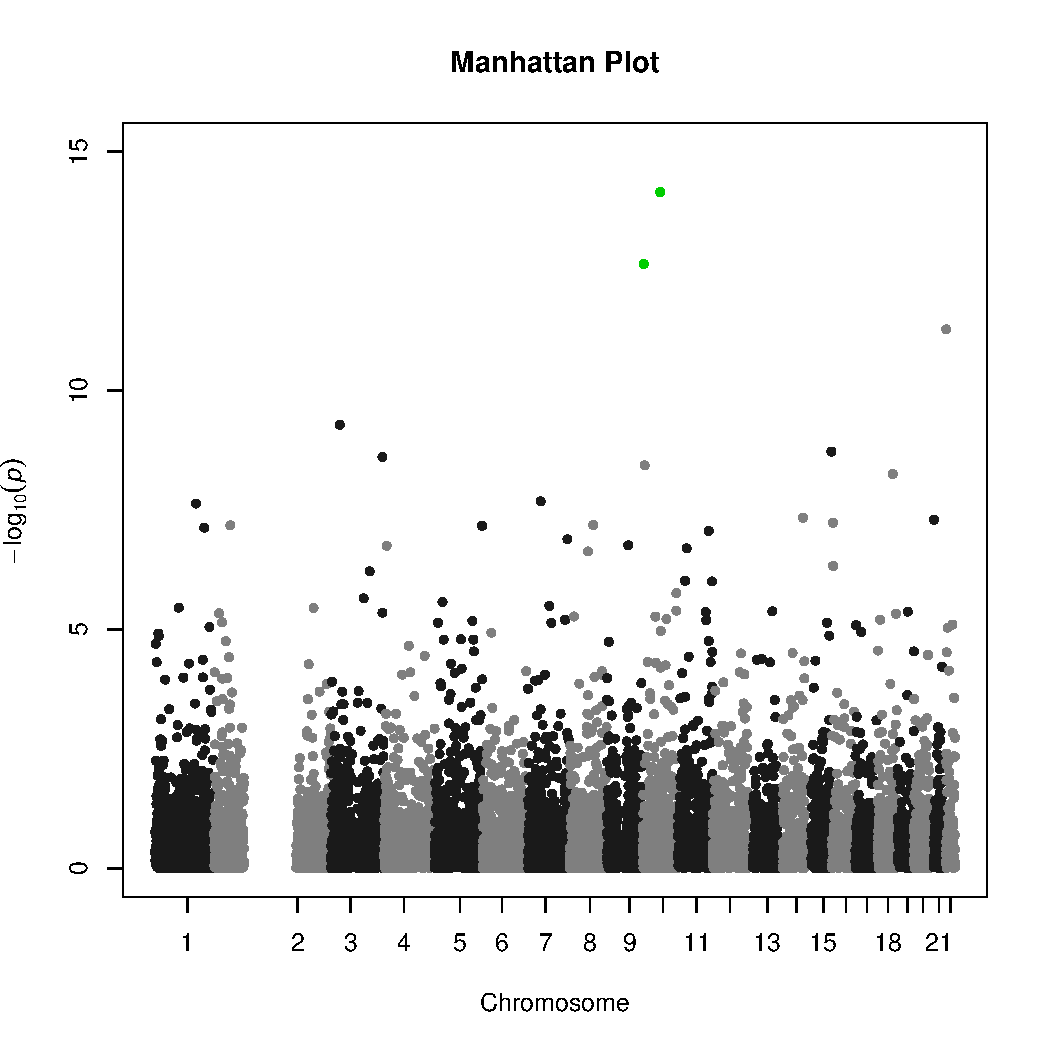
\includegraphics[width=18cm,height=18cm]{manhattan.pdf}}

\section{Contact}
If you need assistance, do not hesitate to send me an
email (efrichot@gmail.com). 
A FAQ (Frequently Asked Questions) section is available 
on our webpage (ttp://membres-timc.imag.fr/Olivier.Francois/lfmm.html). 
LFMM software is still under development. 
All your comments and feedbacks are more than welcome.

\bibliography{biblio}
\bibliographystyle{plain}

\end{document}
